% !TeX spellcheck = it_IT
\documentclass{article}
\usepackage[T1]{fontenc}
\usepackage[utf8]{inputenc}
%\usepackage[italian]{babel}
\usepackage[paper = a4paper, margin = 1in]{geometry}
\usepackage{graphicx}
\usepackage{amsfonts, epsfig}
\usepackage[hyphens]{url}
\usepackage{hyperref}
\usepackage{amssymb}
\usepackage{listings, lstautogobble}
\usepackage[export]{adjustbox}[2011/08/13]
\usepackage{verbatim}
\usepackage{subfig}
\usepackage{media9}
\usepackage{graphicx}
\usepackage{pxfonts}
\usepackage{tabularx}
\usepackage[dvipsnames]{xcolor}
\usepackage{textcomp}
\usepackage{eurosym}

\lstset{
	breaklines = true,
	autogobble = true
}
\AtBeginDocument{\AtBeginShipoutNext{\AtBeginShipoutDiscard}}

\lstset{language = C,
	basicstyle = \ttfamily,
	keywordstyle = \bfseries,
	showstringspaces = false,
	literate = {:=}{$\leftarrow{}$}{1},
	morekeywords = {foreach, repeat, until, function, return, end, in, do, new, private, public, protected, internal, string, class, overridenu}
}

\renewcommand*\contentsname{Indice}

\newenvironment{nscenter}
{\parskip =0 pt\par\nopagebreak\centering}
{\par\noindent\ignorespacesafterend}

\renewcommand{\listfigurename}{Elenco delle Figure}

\renewcommand{\listtablename}{Elenco delle Tabelle}

\begin{document}
	\title{
		\pagenumbering{gobble}	
		% Frontespizio	
		\begin{titlepage}
			\centering
			
			{\huge\bfseries \textsc{Manuale} \par}
			\vspace{2cm}					
		\end{titlepage}
	}

	\maketitle
	
	% Indice
	\pagenumbering{roman}
	
	\tableofcontents
	\newpage
	
	\listoffigures
	\newpage
	
	\listoftables
	\newpage
	
	\pagenumbering{arabic}
	
	\newgeometry{top = 1in, bottom = 1in, right = 0.8in, left = 0.8in}
	\maketitle
	\newpage
	
	\section{Introduzione al framework} \label{section:Introduzione}
		Il framework è composto dai seguenti gruppi logici:
		
		\begin{itemize}
			\item Core
			\item Diagnostic
			\item Extensions
			\item Hardware
			\item IO
			\item Mathematics
			\item Signal
			\item Devices
			\item Benches
			\item Instructions
			\item User interface
		\end{itemize}
		
		Ognuno di questi gruppi può essere a sua volta suddiviso in dei sottogruppi specializzati nell'implementare una singola funzionalità. In linea di massima il framework cerca di lavorare il più possibile con una logica ad eventi in modo da alleggerire l'overhead richiesto per la scrittura di codice ad alto livello.
		
		\paragraph*{}
		Nelle sezioni seguenti verranno meglio descritti i vari gruppi logici appena riportati e, per ognuno di essi, si scenderò poi nel dettaglio dei vari namespace in essi contenuti, facendo quindi riferimento al codice effettivamente implementato per ogni funzionalità.
		\par
		L'ordine con cui verranno esposti (e sono stati riportati in questa sezione) i gruppi e il codice segue un andamento dall'alto verso il basso, ovvero partendo da nucleo del framework (Core), passando l'hardware e funzionalità di input/output (Hardware e IO), fino ad arrivare a dispositivi e banchi (Devices e Benches con le relativi istruzioni, ovvero Instructions), per finere con l'interfaccia grafica (UserInterface).
		\newline
		Nel mezzo sono presenti altri gruppi di supporto (quali, ad esempio, Diagnostic piuttosto che Extensions, Mathematics o Signal).
	\newpage
	
	\subsection{Schema di massima dell'architettura del framework}
		I dettagli dei vari e gruppi logici verranno descritti in seguito, mentre in questa sezione viene riportato lo schema logico di massima dell'organizzazione dei vari blocchi che compongono il framework, partendo dal basso verso l'alto e come questi dovrebbero interagire.
		
		\begin{figure}[htbp]
			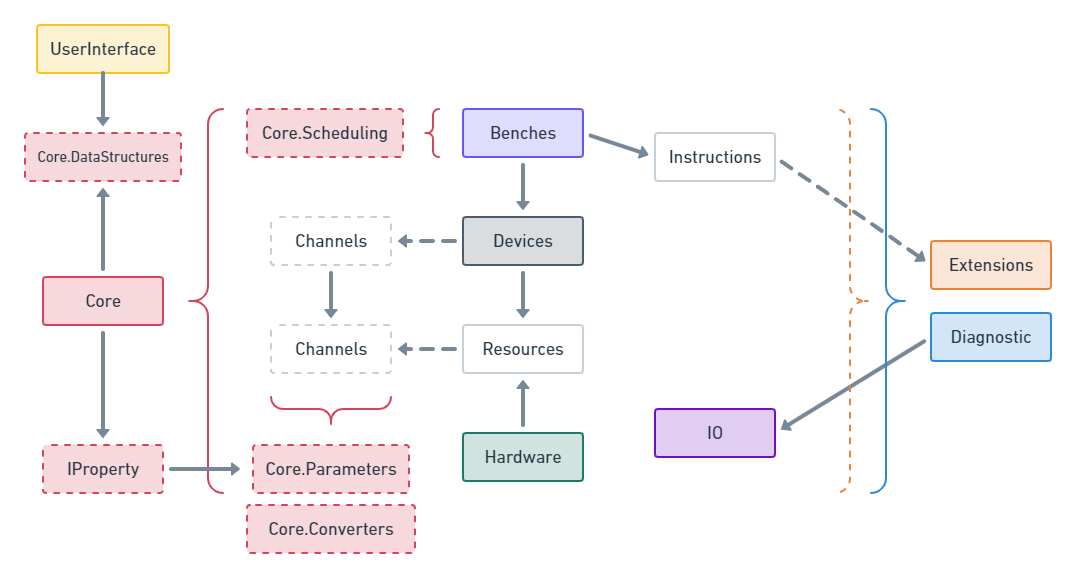
\includegraphics[width=1\textwidth, center] {img/framework_logic_scheme.png}
			\caption[Schema logico del funzionamento del framework]
			{Schema logico di funzionamento di massima del framework, con le varie interazioni di base tra i vari elementi che lo compongono. \label{fig:frameworkLogicScheme}}
		\end{figure} 
		
		\paragraph*{Core}
		Come si può vedere dall'immagine, il nucleo principale del framework è rappresentato dal namespace Core, che verrà richiamato dai vari altri livelli dell'architettura (se non direttamente come "sotto-namespace" di Core, come ad esempio Core.Scheduling o Core.DataStructures).
		\newline
		Mentre una descrizione più approfondita di Core verrà data in seguito, a questo livello basta dire che, ad esempio, in Core (raggruppando in esso anche i namespace derivati) è presente la classe (statica) ServiceBroker, che conterrà, a run-time, la collezione con tutti gli oggetti (o servizi) ad esso aggiunti (quindi, ad esempio, conterrà l'insieme di tutti i canali sottoscritti, in modo da permetterne il recupero e l'utilizzo in modo agevole in tutte le parti del codice).		
		\par
		Definito a grandi linee il namespace Core, occorre ora introdurre l'interfaccia (contenuta in Core) IProperty: questa funge da prototipo di base per ogni tipo di classe successiva del framework; ogni classe che fa riferimento, ad esempio, ad un canale o una risorsa, deriverà, in modo diretto o indiretto, da IProperty o eventualmente dalla versione con generics dell'interfaccia IProperty$<$T$>$ (con quest'ultima che comunque a sua volta deriva da IProperty).
		\newline
		In altre parole, quindi, si può dire che IProperty è l'elemento più generale del framework.
		
		\paragraph*{Hardware}
		Al livello successivo troviamo il namespace Hardware che conterrà definizioni generiche legate all'hardware (ad esempio si avrà l'interfaccia IResource, che funge da base per le varie risorse fisiche, oltre che la definizione dei vari canali hardware di input/output, sia digitali che analogici), che a sua volta contiene N namespace, ognuno riferito ad una risorsa fisica (come precedentemente accennato) quali ad esempio quella per comunicare tramite protocollo modbus, seriale, tcp, ecc.
		
		\paragraph*{Devices}
		Proseguendo, si avrà il namespace per la gestione dei device (che potrebbero essere, ad esempio, un alimentatore piuttosto che uno strumento di acquisizione). Questo livello si appoggia direttamente sull'hardware per la parte di gestione della comunicazione ed implementerà la logica di gestione dei dispositivo fisico (come ad esempio l'accensione e l'impostazione di una tensione per l'alimentatore).
		\newline
		La comunicazione con la risorsa hardware sottostante può avvenire tramite il metodo ConnectTo, definito nella classe generica Channel. Eseguendo ad esempio l'istruzione:
		
		\begin{lstlisting}
			AnalogInput x = new AnalogInput();
			AnalogInput y = new AnalogOutput();
			.
			.
			.
			x.ConnectTo(y);
		\end{lstlisting}
	
		ad ogni cambiamento del valore del canale x, questo si propagherà anche al canale y (e a tutti quelli così sottoscritti). In aggiunta, è anche possibile specificare una Action da eseguire in fase di propagazione del valore ed effettuare quindi una conversione (tramite l'oggetto sotto definito di tipo GenericConverter). Ad esempio:
		
		\begin{lstlisting}
			AnalogInput x = new AnalogInput();
			AnalogInput y = new AnalogOutput();
			double convertionFactor = 0.5;
			.
			.
			.
			x.ConnectTo(
				y,
				new GenericConverter<double, double>(
					(x) => x * conversionFactor
				)
			);
		\end{lstlisting}
		
		moltiplicherà il valore di x per 0.5 e lo assegnerà ad y (con il valore di x che, in questo processo, non viene modificato: se ad esempio x = 2, alla fine dell'istruzione x sarà ancora uguale a 2, mentre y avrà valore 1).
	\newpage
	
	\section{Core} \label{section:Core}
	
	\newpage
	
	\subsection{Parameters} \label{subsection:Parameters}
		
	\newpage
	
	\subsection{Converters} \label{subsection:Converters}
	
	\newpage
	
	\subsection{DataStructures} \label{subsection:DataStructures}
	
	\newpage
	
	\section{Diagnostic} \label{section:Diagnostic}
	
	\newpage
	
	\section{Extensions} \label{section:Extensions}
	
	\newpage
	
	\section{Hardware} \label{section:Hardware}
	
	\newpage
	
	\section{IO} \label{section:IO}
	
	\newpage
	
	\section{Mathematics} \label{section:Mathematics}
	
	\newpage
	
	\section{Signal} \label{section:Signal}
	
	\newpage
	
	\section{Devices} \label{section:Devices}
	
	\newpage
	
	\section{Benches} \label{section:Benches}
	
	\newpage
	
	\section{Instructions} \label{section:Instructions}
	
	\newpage
	
	\section{UserInterface} \label{section:UserInterface}
		
	\newpage
	
	\section{Utilizzo del framework} \label{section:Utilizzo}
		Per l'utilizzo del framework si può fare riferimento al progetto BaseProject, che contiene lo scheletro di massima dell'applicazione grafica contenente tutti i pannelli generali e l'inizializzazione di alcuni componenti standard del framework (quali, ad esempio, il ServiceBroker o il Logger). Il progetto GetStarted, invece, fa riferimento ad un esempio di utilizzo del framework con dell'hardware (un Arduino in questo caso per utilizzare la comunicazione seriale e quindi la classe SerialResource) in modo da mostrare l'utilizzo di tutti gli strati messi a disposizione dal framework, anche se in una modalità semplificata e con un hardware minimo
		\par
		L'inizializzazione del framework viene fatta all'interno del metodo InitializeFramework, in cui si avrà il seguente codice:
		
		\begin{lstlisting}
			private static void InitializeFramework()
			{
				// Initialize the logger
				Logger.Initialize();
				Logger.SetMinimumSeverityLevel(Severity.Trace);
				Logger.Log("Logger initialized", Severity.Trace);
				
				// Enable the logger to acquire all the generated exceptions
				AppDomain.CurrentDomain.FirstChanceException += (sender, eventArgs) =>
				{
					Logger.Log(eventArgs.Exception);
				};
				Logger.Log("Started exception intercept service", Severity.Trace);
				
				// Start the log reader
				LogReader.StartRead();
				Logger.Log("Log reader started for diagnostic", Severity.Trace);
				
				// Initialize the service broker
				ServiceBroker.Initialize();
				Logger.Log("ServiceBroker initialized", Severity.Trace);
				
				// Initialize the scripting functionalities
				InitializeScripting();
				
				// Initialize the user interface
				InitializeUserInterface();
				Logger.Log("User interface initialized", Severity.Trace);
				
				Logger.SetMinimumSeverityLevel(Severity.Info);
				Logger.Log("Framework initialized", Severity.Info);
			}
		\end{lstlisting}
	
		\newpage
	
		Particolare importanza rivestono i metodi InitializeScripting e InitializeUserInterface presenti nel codice appena riportato: nel primo metodo andranno creati tutte le varie classi che derivano da Script da utilizzare nell'applicazione, mentre nel secondo dovranno essere aggiunti tutti i controlli relativi all'interfaccia grafica.
		\newline
		Di seguito vengono riportati due esempi di aggiunta di elementi in fase di inizializzazione. Nel primo si fa riferimento al metodo InitializeScripting, in cui viene aggiunto un SerialCatalog alla collezione contente tutti gli oggetti di classi derivanti da Script; nel secondo, invece, viene mostrato il metodo InitializeUserInterface in cui si può vedere come aggiungere un nuovo elemento  all'interfaccia grafica.
		
		\begin{lstlisting}
			private static void InitializeScripting()
			{
				// Add here all the scripts creation:
				_ = new SerialCatalog("MainCatalog"); // Example
				
				ScriptManager.Initialize();
				Logger.Log("ScriptManager initialized", Severity.Trace);
				
				ScriptManager.ExecuteScripts();
				Logger.Log("Scripts executed", Severity.Trace);
			}
		\end{lstlisting}
	
		\begin{lstlisting}
			private static void InitializeUserInterface()
			{
				controls = new List<BaseControl>();
				
				controls.Add(new AutomaticPanel("Automatic"));
				controls.Add(new ManualPanel("Manual"));
				controls.Add(new DiagnosticPanel("Diagnostic"));
				controls.Add(new InfoPanel("Info"));
			}
		\end{lstlisting}
		
		\newpage
		
		Per quanto riguarda la creazione di nuovi Script da aggiungere in fase di inizializzazione, di seguito è riportato un esempio:
		
		\begin{lstlisting}
			public class SerialCatalog : Script
			{
				private SerialResource resource;
				private SerialOutput output;
				private SerialInput input;
				
				private ArduinoDevice device;
				
				private ArduinoBench bench;
				
				public SerialCatalog(string code) : base(code)
				{
					resource = new SerialResource("SerialResource", "COM3");
					resource.Start();
					
					output = new SerialOutput("SerialOutput", "", resource);
					input = new SerialInput("SerialInput", "p", resource);
					
					device = new ArduinoDevice("ArduinoDevice");
					
					ServiceBroker.Add<IResource>(resource);
					ServiceBroker.Add<IChannel>(output);
					ServiceBroker.Add<IChannel>(input);
					ServiceBroker.Add<IDevice>(device);
					
					bench = new ArduinoBench("ArduinoBench");
					
					StringParameter command = (device.Parameters.Get("Command") as StringParameter);
					command.ConnectTo(output);
					StringParameter potentiometer = device.Parameters.Get("Potentiometer") as StringParameter;
					input.ConnectTo(potentiometer);
				}
				
				public override void Execute()
				{
					ServiceBroker.Add<IBench>(bench);
				}
			}
		\end{lstlisting}
		
		Si può notare come in questo codice di esempio vengono creati il device, il bench e tutti i vari channel necessari all'applicazione e vengono poi aggiunti al ServiceBroker, in modo da poter essere recuperati in seguiti in altre parti del programma in caso di bisogno. Occorre notare che nella classe dell'esempio è presente il metodo Execute (override): tale metodo verrà eseguito dallo ScriptManager (gli script vengono aggiunti in automatico nel metodo costruttore della classe Script, per cui è importante che ogni classe che derivi da questa abbia il riferimento al base(code) nel metodo costruttore, come riportato nell'esempio).
		\newline
		Per quanto riguarda invece l'interfaccia grafica e l'aggiunta di nuovi pannelli, questo può essere fatto come riportato precedentemente nell'esempio. Per la creazione del singolo pannello, basta derivare dalla classe PanelControl. Al momento della creazione della classe così derivata, è necessario associare al nuovo controllo un codice (univoco) e aggiungere l'oggetto così creato alla lista controls (già dichiarata all'interno del file Program.cs del progetto). Tale collezione di oggetti verrà passato come parametro al costruttore della classe MainForm, che provvederà ad aggiungere tutti i controlli presenti e a visualizzarli nella form principale del programma (i controlli di default quali quello manuale).
	\newpage
\end{document}
